\section{Einleitung}
Modelle der echten Welt, wie sie in Anwendungen der Künstliche Intelligenz und wissensbasierten Systemen zu finden sind, können nie exakt die Realität abbilden. Durch Messfehler, Subjektivität oder schlichtweg fehlende Kenntnis von Parametern entsteht eine unscharfe Abbildung, die entsprechend behandelt werden muss. Neben der Evidenztheorie von Arthur P. Dempster bieten sich dafür vor allem probabilistische Methoden wie Bayes-Netze an. Diese kennen Fakten nicht nur in binärer Logik, sondern können Werte zwischen wahr und falsch mit statistischen Methoden modellieren.

Dieser Projektbericht beschreibt den Entwurf und die Umsetzung eines Programms zur Vorhersage eines Versicherungstarifs basierend auf Personendaten mithilfe eines Bayes-Netzes und bewertet die Ergebnisse anschließend.


\section{Entwurf}
Für diesen Programmentwurf ist ein Datensatz mit Angaben zu Personen gegeben, von denen 5 Spalten kategorisch (Geschlecht, Familienstand, Bildungsstand, Beruf, Immobilienbesitz) und 3 Spalten numerisch (Alter, Kinder, Jahresgehalt) sind. Der Datensatz enthält außerdem den vergebenen Versicherungstarif (Tarif A--B oder abgelehnt) zu diesen Personen. Zur Verwendung in einem Bayes-Netz müssen numerische Spalten durch \textit{binning} in Kategorien eingeteilt werden, um darauf Wahrscheinlichkeitstabellen erstellen zu können. Die Wahl der Grenzen zwischen den Kategorien ist eine Abwägung zwischen Verallgemeinerung (wenige Kategorien) und Aussagekraft (viele Kategorien). Dafür haben wir die Daten visuell in einem Jupyter-Notebook (zu finden unter \texttt{data/exploration.ipynb}) untersucht und uns für folgende Einteilung entschieden:
\begin{itemize}
    \item Alter: 0--20, 20--40, 40--80, 80--100
    \item Jahresgehalt (in Tausend): 0--20, 20--40, 40--60, 60--80, 80--100, 100--120, 120--140
    \item Kinder: 0, 1, 2, 3, 4, 5, 6, 7, 8
\end{itemize}

Die Verwendung des Bayes-Netzes soll in einer Klasse \texttt{InsuranceAdvisor} verpackt werden, um die Schnittstelle einfach zu halten und das domänenspezifische Wissen über die Versicherungsdaten zu kapseln. Die Klasse braucht folgende Methoden:
\begin{itemize}
    \item \texttt{load\textunderscore data}: Daten aus .csv-Datei laden, validieren und transformieren
    \item \texttt{fit}: Modell mit Trainingdaten trainieren
    \item \texttt{predict}: Vorhersage für Versicherungstarif anhand des Modells treffen
    \item \texttt{predict\textunderscore probabilities}: Vorhersage für Wahrscheinlichkeit aller Versicherungstarife treffen
    \item \texttt{save\textunderscore model}: Modell in Datei speichern
    \item \texttt{load\textunderscore model}: Modell aus Datei laden
\end{itemize}
Dies entspricht auch der Schnittstelle für Classifier in \texttt{scikit-learn}, somit können Bewertungsmethoden aus diesem Package verwendet werden.


\section{Implementierung}
Zur Umsetzung wählen wir Python 3, da es hierfür eine Vielzahl an Bibliotheken gibt, um schnell eine funktionierende Lösung zu erstellen. Insbesondere verwenden wir das Package \texttt{pomegranate}, das eine Reihe an probabilistischen Modellen inklusive Bayes-Netzen enthält. \texttt{pomegranate} kann die Graph-Struktur und Conditional Probability Tables eines solchen Netzes von Beispieldaten lernen und für diverse Formen probabilistischer Inferenz (diagnostisch, kausal, interkausal, gemischt) anwenden. Dabei werden notwendige Bedingungen wie Azyklizität und P-Separierbarkeit eingehalten. Wir verwenden die A*-Variante\footnote{\url{https://github.com/jmschrei/pomegranate/blob/master/pomegranate/BayesianNetwork.pyx#L1558-L1646}}. Die Benutzung des Packages wird dann in der Klasse \texttt{InsuranceAdvisor} gekapselt.

Zusätzlich gibt es ein Skript, das den gesamten Datensatz in Trainings- und Testdaten zufällig im Verhältnis 70:30 aufteilt und in separaten Dateien im  Ordner \texttt{data/} speichert. Dabei wird sichergestellt, dass in den Trainingsdaten jeder Wert für die Spalte Kinder einmal vorkommt. Andernfalls treten Probleme auf, wenn eine Kategorie dem Netz nicht bekannt ist. Außerdem werden die ersten 10 Testdaten ohne Versicherungstarif in einer weiteren Datei gespeichert, um Inferenz testen zu können.


\section{Verwendung}
Zur Verwaltung von Abhängigkeiten und der Python-Umgebung verwenden wir \texttt{pipenv}, welches wie hier\footnote{\url{https://pipenv.kennethreitz.org/en/latest/install/#installing-pipenv}} beschrieben installiert werden kann. Dann kann die Umgebung per \texttt{pipenv install -{}-skip-lock} eingerichtet und per \texttt{pipenv shell} im obersten Ordner aktiviert werden. Ohne Verwendung der \texttt{pipenv}-Shell kommt es zu Abhängigkeitsproblemen. Unser Programm kann dann per Aufruf der folgenden Befehle, und insbesondere der funktionierenden Beispiele, in dieser Shell ausgeführt werden. Es bietet drei Modi.

\subsection{Training}
Aufruf: \texttt{python insurance\textunderscore advisor train [train-data]} \\
Beispiel: \texttt{python insurance\textunderscore advisor train data/dataset\textunderscore train.csv} \\
Daten: Features + Versicherungstarif \\
Mit diesem Befehl wird das Bayes-Netz aus den Trainingsdaten erlernt und im Ordner \texttt{model/} gespeichert. Die Datei mit Trainingsdaten muss dabei alle Spalten enthalten. Außerdem wird die Modell-ID ausgegeben, die in den anderen Modi verwendet werden kann.

\subsection{Vorhersage}
Aufruf: \texttt{python insurance\textunderscore advisor predict [model-id] [predict-data]} \\
Beispiel: \texttt{python insurance\textunderscore advisor predict default data/dataset\textunderscore predict.csv} \\
Daten: Features \\
Mit diesem Befehl wird der Versicherungstarif für neue Daten vorhergesagt und mit einer Wahrscheinlichkeit als Tabelle ausgegeben. Dafür wird wieder die Modell-ID eines vorher trainierten Modells, wie etwa aus dem letzten Schritt, und der Pfad zu einer Datei mit Daten angegeben. Die Daten müssen alle Spalten enthalten, allerdings dürfen davon beliebige Einträge leer sein.

\subsection{Evaluation}\label{sec:evaluation}
Aufruf: \texttt{python insurance\textunderscore advisor evaluate [model-id] [test-data]} \\
Beispiel: \texttt{python insurance\textunderscore advisor evaluate default data/dataset\textunderscore test.csv} \\
Daten: Features + Versicherungstarif \\
Mit diesem Befehl werden Testdaten vorhergesagt und die vorhergesagten und wahren Versicherungstarife verglichen. um Klassifikationsmetriken und eine Confusion Matrix zu generieren. Dafür wird die Modell-ID eines vorher trainierten Modells und der Pfad zu einer Datei mit Testdaten angegeben.


\section{Bewertung}
\begin{figure}[b!]
    \captionsetup[subfigure]{justification=centering}
    \centering
    \begin{SubFloat}{Metriken\label{fig:metrics}}%
    \footnotesize
    \begin{minipage}[b]{0.45\linewidth}% 
    \begin{BVerbatim}[baselinestretch=.9]
       precision recall f1-score support

 Tarif A    0.86   0.81   0.84    107
 Tarif B    0.77   0.87   0.82    119
 Tarif C    0.89   0.48   0.63     33
 Tarif D    1.00   1.00   1.00      4
ablehnen    0.86   0.97   0.91     37

accuracy                  0.82    300
    \end{BVerbatim}%
    \vspace{4em}
    \end{minipage}%
    \end{SubFloat}
    \quad
    \subfloat[Nicht normalisiert\label{fig:cmatrix1}]{
        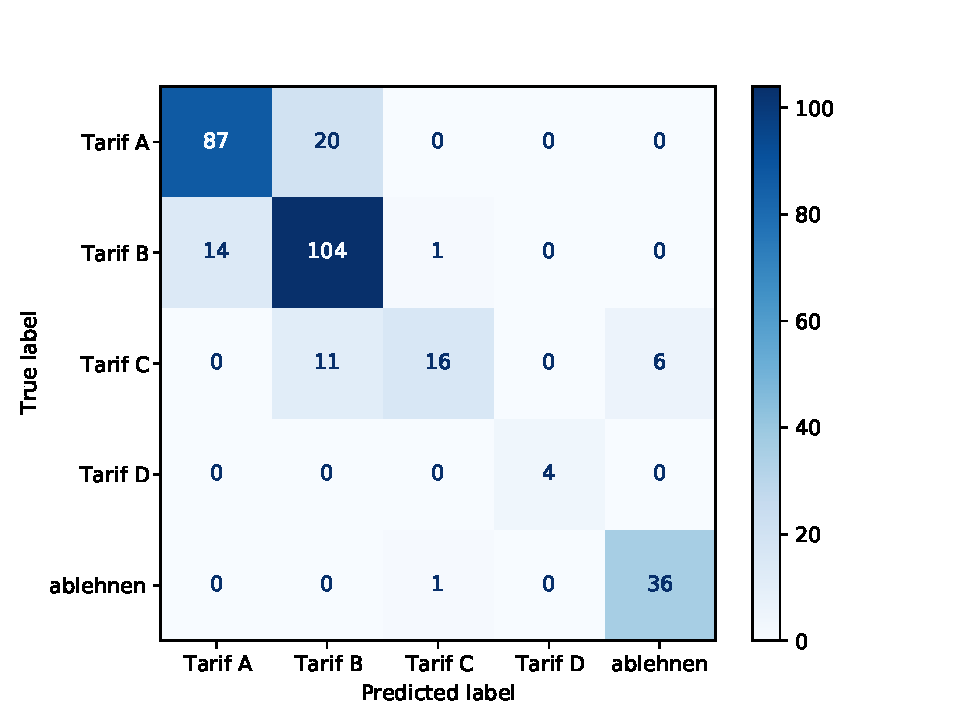
\includegraphics[width=0.45\linewidth]{img/confusion_matrix.pdf}
    }
    
    \subfloat[Normalisiert über wahres Label \\ Precision auf der Diagonalen\label{fig:cmatrix2}]{
        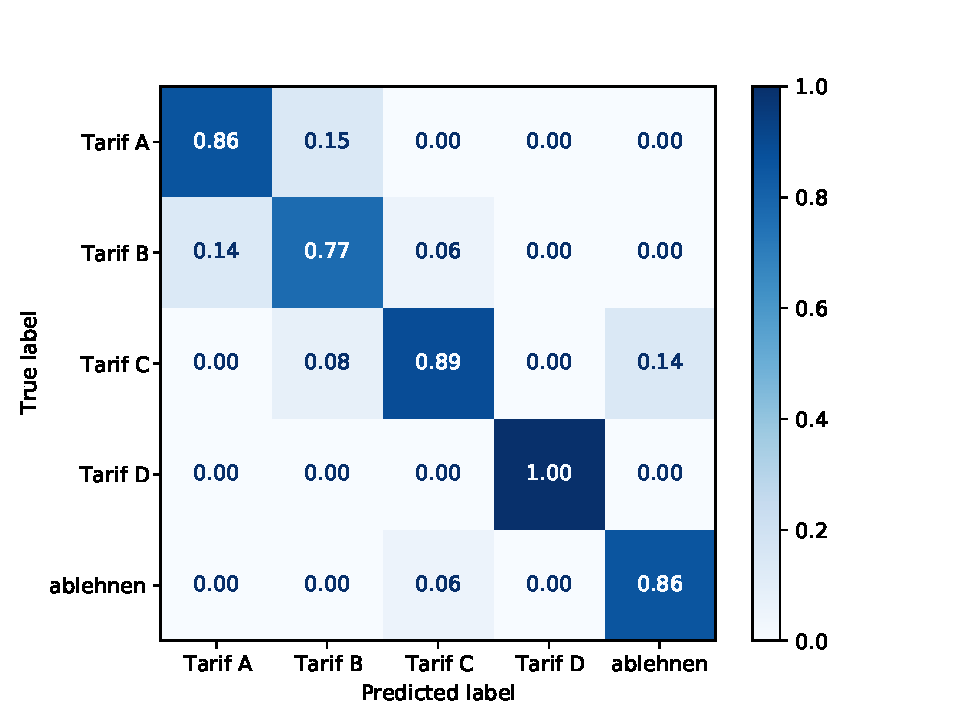
\includegraphics[width=0.45\linewidth]{img/confusion_matrix_precision.pdf}
    }
    \quad
    \subfloat[Normalisiert über vorhergesagtes Label \\ Recall auf der Diagonalen\label{fig:cmatrix3}]{
        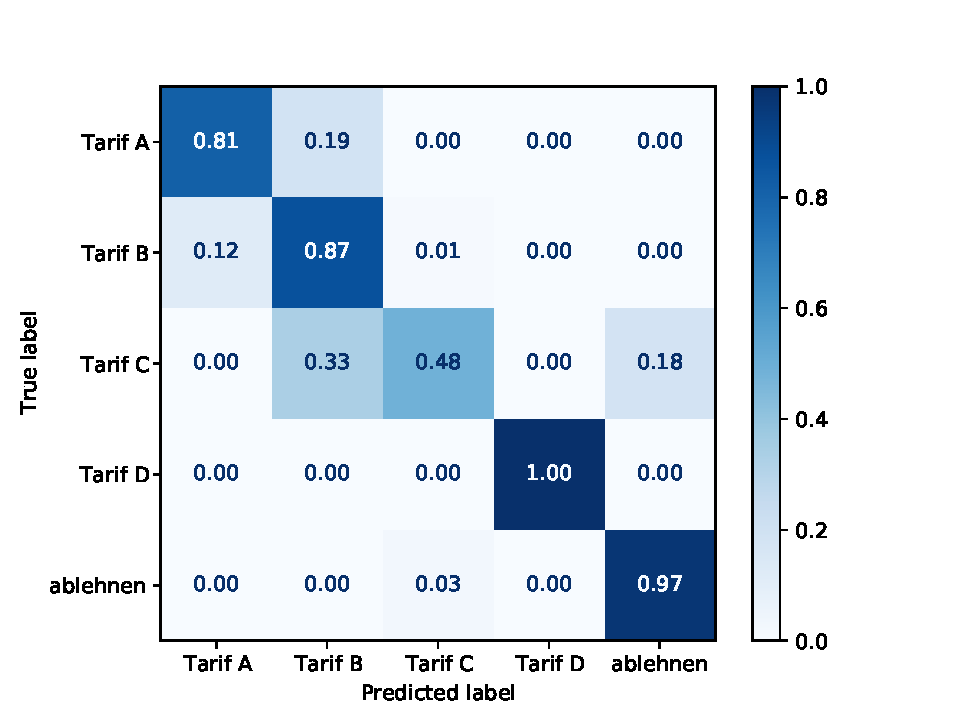
\includegraphics[width=0.45\linewidth]{img/confusion_matrix_recall.pdf}
    }
    
    \caption{Klassifikationsergebnisse}
\end{figure}

Zur Bewertung der Klassifikation haben wir unser Modell mit den Testdaten aus dem Train/Test-Split mit dem Befehl aus Abschnitt \ref{sec:evaluation} ausgeführt. Die Metriken sind in Abbildung \ref{fig:metrics} dargestellt. Außerdem sind die Ergebnisse in Form von drei Confusion Matrices abgebildet. Abbildung \ref{fig:cmatrix1} ist eine übliche Confusion Matrix mit absoluten Angaben. Abbildung \ref{fig:cmatrix2} und \ref{fig:cmatrix3} zeigen die selben Daten wie \ref{fig:cmatrix1}, allerdings pro Kategorie über die wahren Labels beziehungsweise über die vorhergesagten Labels normalisiert. Dadurch sind Precision beziehungsweise Recall auf der Diagonalen ablesbar. Durch die Normalisierung lassen sich die Versicherungstarife untereinander vergleichen, obwohl unterschiedliche viele Beispiele für verschiedene Tarife vorliegen.

Wir erreichen eine Accuracy, also einen Anteil insgesamt korrekt klassifizierter Einträge, von 82\%. Etwa in diesem Bereich bewegen sich auch Precision, Recall und F1-Scores aller Tarife. Nur Tarif C hat mit 48\% einen deutlich schlechteren Recall, denn er wird in 33\% aller Fälle als Tarif C klassifiziert. Auch zwischen Tarif A und B gibt es einige Verwechslungen. Tarif C, Tarif D und Ablehnungen sind in den Testdaten allerdings nur wenig vorhanden, daher ist die Signifikanz der Ergebnisse für diese Kategorien eher gering.

Der von \texttt{pomegranate} automatisch generierte Graph des Bayes-Netzes ist in Abbildung \ref{fig:bayesnet} dargestellt. Es ist deutlich zu sehen, dass der Versicherungstarif zentral liegt und direkt von fünf Features abhängt. Während Zusammenhänge wie Beruf $\xrightarrow{}$ Jahresgehalt $\xrightarrow{}$ Immobilienbesitz logisch plausibel sind, wäre man manuell wohl nicht auf diese Graph-Struktur gekommen.

\begin{figure}
    \centering
    \includegraphics[width=\linewidth]{img/graph.pdf}
    \caption{Grafische Darstellung des Bayes-Netzes}
    \label{fig:bayesnet}
\end{figure}


\newpage
\section{Zusammenfassung}
In diesem Bericht haben wir unseren Programmentwurf zur Vorhersage von Versicherungstarifen mit Bayes-Netzen vorgestellt. Dabei nutzen wir das Erlernen der Graph-Struktur und Wahrscheinlichkeitsverteilungen durch \texttt{pomegranate} und erreichen zufriedenstellende Ergebnisse. Das Programm ist über eine Kommandozeilen-Schnittstelle zu bedienen.

Das Modell könnte in einem realen Szenario als Empfehlung für einen menschlichen Berater dienen, allerdings sollte es nicht selbstständig für Entscheidungen verantwortlich sein. Außerdem sollte es auf Voreingenommenheit gegenüber diversen Personengruppen geprüft werden. Andere Methoden des maschinellen Lernens wie Random Forests, Gradient Boosted Trees oder Support Vector Machines könnten möglicherweise bessere Ergebnisse liefern und sollten als Alternativen in Erwägung gezogen werden.
